	\section{View}
		%\begin{enumerate}
	\subsection{Allgemein}
		%Einleitung
		Kommen wir nun zum nächsten Großen Abschnitt des Programm-Entwurfs.
		Nachdem wir im letzten Abschnitt über das Model gesprochen haben folgt nun der View-Teil des "Model-View-Controller"-Entwurfsmusters.
		Die View beschäftigt sich, wie der Name andeutet mit dem Aussehen des Programms und somit mit der graphischen Repräsentation.
		
		%Überleitung:
		Wie im Pflichtenheft beschreiben haben wir uns für die Entwicklung mit Java entschieden.
		Unter Java gibt es mehrere Möglichkeiten eine GUI zu erstellen.
			
			\begin{enumerate}
				\item Standart Widget Toolkit (SWT)
				\item Abstract Widget Toolkit (AWT)
				\item Swing
				\item JavaFx
			\end{enumerate}

		Uns war allerdings relativ schnell klar, dass die Wahl auf JavaFx fallen wird.
		Dies lag nicht zuletzt an FXML und der bisherigen Entwicklungs-Erfahrung.
		Dazu gleich mehr.
		
			\subsubsection{JavaFX}
			%Allgemeine Beschreibung:
			\begin{itemize}
			\item JavaFX ist eine Abkürzung für Java Graphics.
			\item JavaFX ist eine Möglichkeit unter Java eine graphische Oberfläche zu erstellen.
			\item JavaFX ist eine komplette Neuentwicklung von Oracle.
			\item Es ist unabhängig von den bisherigen Methoden AWT und Swing.
			\item JavaFX wurde 2014 veröffentlicht.
			\item Es ist seit Version 7.6 in x86 Java Standard Edition (JavaSE) Runtime Installation enthalten.
			\item Da wir mit Java 8 arbeiten werden ist dies somit kein Problem.
			\end{itemize}
			
			%Aufbau
			JavaFX arbeitet mit einem Szenengraphen (engl. scene graph), der die einzelnen Bestandteile einer GUI verwaltet.
			Auf diesen werden dann alle weiteren Bestandteile gesetzt.
			
			\subsubsection{FXML}
				%Einleitung:
				Wie auch bei den alternativen kann man natürlich auch mit JavaFx über zu schreibenden Code GUI-Objekte erstellen und diese auf den Scenen-Graphen aufbringen.
				Allerdings besteht mit JavaFx erstmals die Möglichkeit eine neue Form der GUI Entwicklung zu beschreiten.
				Diese erfolgt in Form von FXML.
				
				%Allgemeine Beschreibung:
				FXML ist eine deklarative Beschreibung der grafischen Oberflächen auf XML-Basis.
				Dies bietet einige Vorteile gegenüber der konventionellen GUI-Entwicklung.
				Zum einen ist durch diese Technologie die Trennung des Designs der GUI und deren Funktionalität strikt getrennt.
				Zum anderen ist das Einfügen von GUI-Bestandteilen, die an mehreren Stellen der Benutzeroberfläche zum Einsatz kommen sehr einfach möglich.
				Dies Ermöglicht, dass der mehrfachverwendbare Code nur einmal in einem Separatem FXML-Dokument abgespeichert werden muss und dann über den „include-Tag“ an allen Stellen verwendet werden kann.
				Darüber hinaus können für die Gestaltung auch Web-Technologien wie CSS eingesetzt werden.
				Dies sorgt zusätzlich für eine Trennung von Layout auf der einen und Style und Design auf der anderen Seite, da separate CSS-Dateien erstellt werden können.
				Diese können dann in den FXML-Code eingebettet werden, sodass die GUI das Design übernehmen kann.
				
				%Entwicklung:
				Die Entwicklung der FXML-Dateien erfolgt zuerst über den SceneBuilder.
				Dieser ist ein grafisches Tool, das die Erstellung von FXML-Dateien vereinfacht.
				Der daraus generierte Code wird bei Bedarf dann nochmals per Hand nachbearbeitet.
				Zur Nachbereitung zählen unter anderem auch das Einfügen der „include-Tags“ (wie oben beschrieben).
%			}
	%	}
	
	\subsection{Entwurf}
		%Einführung
		Der Entwurf der View gliedert sich prinzipiell in folgende Pakete auf:
			\begin{enumerate}
				\item Graphic
				\item Drawer
				\item Sound
			\end{enumerate}
		Diese sind Sup-Pakete des "View-Packages" und werden im folgenden genauestens unter die Lupe genommen.

		\mypackage{Graphic}
		The Graphic-Package is a Package for some adaptations and expansions with the JavaFx Stuff.
		
		\mypackage{Graphic.UIElements}
		The UI-Elements-Package contains new created UI-Elements that expand the JavaFx-UI.
		
		\myclass{ZoomableScrollPane}
		
			\textbf{Beschreibung}\newline
			This is an expansion to the JavaFx-ScrollPane.
			This adds the ScrollPane that it can be zoomed.
			
			This is used so that the drawn Graph could be zoomed in/out so that the user can easily look for some Edges.
			
			This Class is not made by ourself.
			@author
			https://www.pixelduke.com/2012/09/16/zooming-inside-a-scrollpane/
			
			\textbf{Dokumentation}\newline
			Because this Class is already fully implemented by the creator, there will be no Documentation from our side.

	\mypackage{Drawer}
	The Drawer-Package.
	This Package contains everything that belongs to the Drawing of the Graphs.
	It is a upper-Package, therefore no further Documentation for this.
	
		\begin{figure}
	\centering
	%\fbox{	
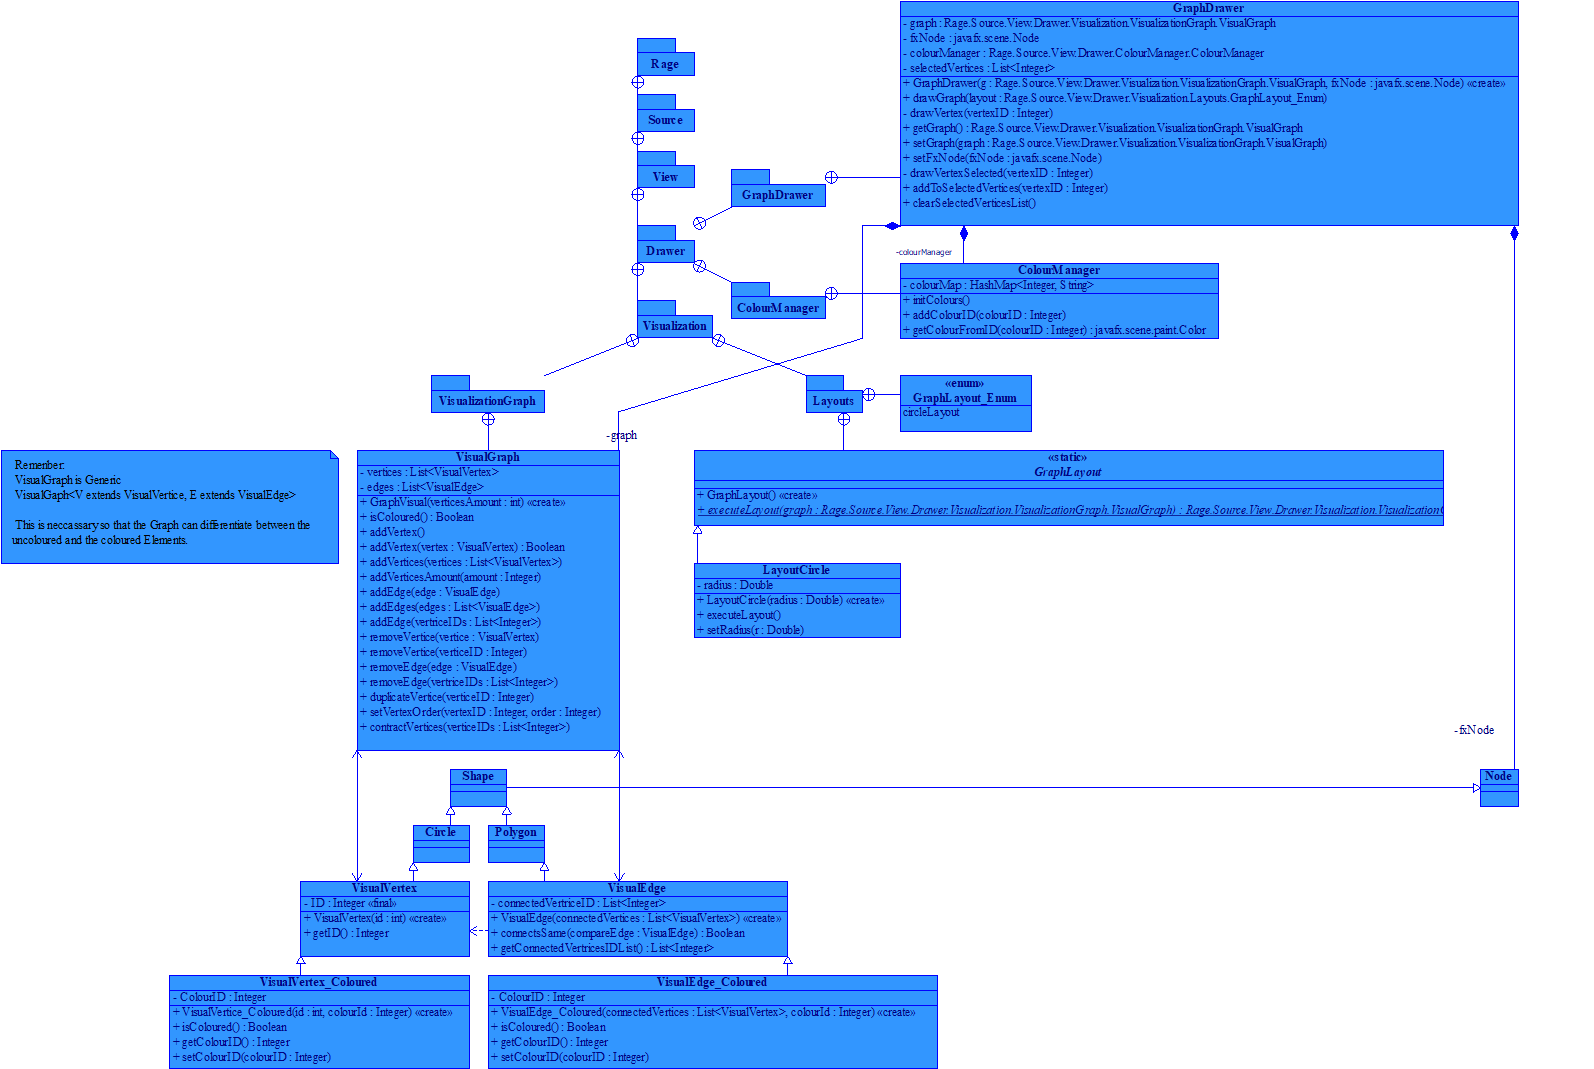
\includegraphics[width=\textwidth]{abbildungen/ClassDiagram_View_Drawer.png}
\caption{ViewDrawer }
	\label{img:viewdrawer}
	\end{figure}
	
	%Hier das ClassDiagram_View_Drawer einfügen.
	
		\mypackage{Drawer.GraphDrawer}
		The GraphDrawer-Package contains like the Name suggested the GraphDrawer that visualizes the Graph and "draws" it to a JavaFx-Node for the User.
		
			\myclass{GraphDrawer}			
				\textbf{Beschreibung}\newline
				The Drawer that draws the given Graph to the given JavaFx-Node.				
				\textbf{Dokumentation}\newline
				\begin{enumerate}[-]
					\item{
						\textbf{graph : VisualGraph} \newline
						The Graph that should be drawn.
					}
					\item{
						\textbf{fxNode : javafx.scene.Node} \newline
						The JavaFx-Node where the Graph should be drawn on.
					}
					\item{
						\textbf{colourManager : ColourManager} \newline
						The ColourManager of this Drawer to Map the ColourID's to the actual Colours of the to drawn Objects.
						
						This Object is created at the Constructor as new ColourManager and before the Drawing the ColourID's are added.
					}
					\item{
						\textbf{selectedVertices : List<Integer>} \newline
						The List of Vertices-ID's that the user selected the Vertices at the GUI.
					}
				\end{enumerate}
				\begin{enumerate}[+]
					\item{
						\textbf{GraphDrawer(graph : VisualGraph, fxNode : javafx.scene.Node)} \newline
						The Constructor of this Class.
						
						Sets the given Graph and fxNode.
						Also initializes the ColourManager.
						\newline
						\textbf{@param graph}
							The Graph that should be set as the Graph of this Drawer.
							\newline
						\textbf{@param fxNode}
							The JavaFx-Node that should be set as the fxNode of this Class.
							\newline
					}
					\item{
						\textbf{printGraphTextual()} \newline
						This Method prints the textual Representation onto the given JavaFx-Node.
						\newline
					}
					\item{
						\textbf{drawGraph(layout : GraphLayoutEnum)} \newline
						This Method draws the Graph to the given JavaFx-Node by using the given Layout to position it's Vertices.
						\newline
						\textbf{@param layout}
							The Enum that indicates which Layout the Drawer should use.
							If it is null the Drawer will use the Circle Layout.
							\newline
					}
					\item[-]{
						\textbf{drawVertex(vertexID : Integer)} \newline
						Draw the given Vertex.
						
						Get the Vertex by searching for the given VertexID at the vertices-List of the given Graph.
						Use the GraphicLayout to get the correct Position of this Vertex.
						\newline
						\textbf{@param vertexID}
							The ID of the to drawn Vertex.
							\newline
					}
					\item[-]{
						\textbf{drawVertexSelected(vertexID : Integer)} \newline
						Draw the given Vertex as a selected Vertex.
						
						This Method is called if the to drawn Vertex of the drawVertex-Method is in the selectedVertices-List.
						
						The Vertex is drawn as selected by adding the corresponding Picture into the Vertex-JavaFx-Shape.
						Then the standard draw-Method is used to do the rest.
						\newline
						\textbf{@param vertexID}
						The ID of the Vertex that should be drawn as a selected Vertex.
						\newline
					}
					\item[-]{
						\textbf{drawEdge(edgePosition : Integer)} \newline
						Draw the Edge that is on the given Position at the Edge-List of the Graph of this Drawer.
						
						This Method only draws one Edge so that the Editor can show specific Edges.
						This Method is also called multiple times to draw all Edges.
						\newline
						\textbf{@param edgePosition}
						The Position of the to drawn Edge at the List of Edges of the Graph.
						\newline
					}
					\item{
						\textbf{addToSelectedVertices(vertexID : Integer)} \newline
						Add the given VertexID to the List of selected ones.
						\newline
						\textbf{@param vertexID}
						The Vertex-ID that should be added to the List of selected Vertices.
						\newline
					}
					\item{
						\textbf{clearSelectedVerticesList()} \newline
						Clear the List of selected Vertices-ID's.
						\newline
					}
					\item{
						\textbf{getGraph() : VisualGraph} \newline
						Get the VisualGraph of this Drawer.
						\newline
						\textbf{@return} returns
							The VisualGraph of this Drawer.
							\newline
					}
					\item{
						\textbf{setGraph(graph : VisualGraph)} \newline
						Set the VisualGraph of this Drawer.
						\newline
						\textbf{@param graph}
							The VisualGraph that should be set.
							\newline
					}
					\item{
						\textbf{setFxNode(fxNode : javafx.scene.Node)} \newline
						Set the JavaFx-Node where the Graph should be drawn on.
						\newline
						\textbf{@param fxNode}
						The  Node that should be set as the JavaFx-Node to draw on.
						\newline
					}
				\end{enumerate}
	
		\mypackage{Drawer.ColourManager}
		The ColourManager-Package.
		This Package only contains the ColourManager which maps the abstract ColourID's that are given by the calculation into a real Colour-Value that could be drawn.
		This Class is separately because it provides a relatively general task, that easily can be (re)used elsewhere.
		
			\myclass{ColourManager}
				\textbf{Beschreibung}\newline
				The ColourManager manages the different Colours by Mapping the ColourID's to an actual Colour-Value, so that the Drawer can draw the coloured Graph by these ColourID's.
				\textbf{Dokumentation}\newline
				\begin{enumerate}[-]
					\item{
						\textbf{colourMap : Hashmap<IntegerString>} \newline
						The HashMap of every ColourID to the actual Colour-Value that is represented as a String.
					}
				\end{enumerate}
				\begin{enumerate}[+]
					\item{
						\textbf{ColourManager()} \newline
						The Empty-Constructor of this Class.
						The Colours are added step by step at a later point.
						\newline
					}
					\item{
						\textbf{ColourManager(colourIDs : List<Integer>)} \newline
						The Constructor of this Class.
						It adds the given ColourID's of the List and puts them into the Hashmap.
						Then the initColours-Method is called so that the mapping is completed for the given ColourId's.
						\newline
						\textbf{@param colourIDs}
							The List of colourID's that should be mapped to real Colour-Values.
							\newline
					}
					\item{
						\textbf{initColours()} \newline
						This Method has to be called when every ColourID is put into the HashMap.
						Then this Method calculates a Assignment of real Colours to the ColourID's and writes them into the HashMap, where it can be read out at a later Time.
						\newline
					}
					\item{
						\textbf{addColourID(colourIDs : Integer)} \newline
						Add a new ColourID to the HashMap, where later the real Colour is mapped to.
						
						It is checked if the given ColourID is already at the HashMap.
						\newline
						\textbf{@param colourIDs}
							The ColourID that should be added.
							\newline
					}
					\item{
						\textbf{getColourFromID(colourID : Integer) : javafx.scene.paint.Color} \newline
						Get the real Colour-Object from the given ColourID.
						This Colour is then used to draw the Vertex/Edge to the screen to represent the Colouring-Solution.
						
						The initColour-Method has to be called first so that the ColourManager has already mapped the Colour-Values at the HashMap.
						\newline
						\textbf{@param colourID}
							The colourID from what the colour should be.
							\newline
						\textbf{@return} returns
							The actual Colour of the Object.
							\newline
					}
				\end{enumerate}
	
		\mypackage{Drawer.Layouts}
		This Package contains the implemented Layouts for the GraphDrawer and the Enum that Lists all of them.
		
			\myclass{GraphLayoutEnum}
				\textbf{Beschreibung}\newline
				This Enum Contains all implemented GraphLayout's that can be used by the graphDrawer to position the VisualVertices.				
				This Enum is needed because the Drawer needs to know whitch Layout to use for the drawing of the Graph and this is done via this Enumeration.				
				In our case there is only one Layout, because we well always draw the Graphs in a Circle.				
				If someone wants to Expand this Drawer by adding a new Layout he/she/it has to update this Enum as well.
				This is not against ObjectOrienting Programming because the Programmer that would add this new Layout already needs to recompile the Program and therefore can expand the Enum as well.
				\textbf{Dokumentation}\newline
				\begin{enumerate}[+]
					\item{
						\textbf{circleLayout} \newline
						The Enum for the possible Layouts.
						
						There will be only one Value in it because we will only use the Circle-Layout.
						But this is needed for possible extensions by other Programmers.
					}
				\end{enumerate}
				
			\myclass{GraphLayout}
				\textbf{Beschreibung}\newline
				This is the Layout of the Drawing of the Graph.				
				It is an abstract class so that there could be multiple Layouts for the Representation that implements this.
				\textbf{Dokumentation}\newline
				\begin{enumerate}[+]
					\item{
						\textbf{GraphLayout()} \newline
						The Constructor of this abstract Class.
						This is used at the Childs if they do not have an separate Constructor because they do not need parameters to set as well.
						\newline
					}
					\item{
						\textbf{executeLayout(graph : VisualGraph) : VisualGraph} \newline
							This is an abstract Method and has to be implemented at the Sub-Classes.
							
							This Method set's the given Graph to the implemented Layout of the particular Child-Class.
							Therefore it sets the Positions of the Vertices of the given Graph.
						\newline
						\textbf{@param graph}
							The Graph that gets the layout set on it.
							Therfore all Elements of this given Graph will be relocated to the calculated Position this Method calculates.
							\newline
						\textbf{@return} returns
							The given Graph with the calculated Layout.
							\newline
					}
				\end{enumerate}
			
			\myclass{GraphLayoutCircle}
				\textbf{Beschreibung}\newline
				This is the Circle Layout of the Graph.
				Therefore this Layout orders the Graph-Nodes into a Circle.
				
				It is an Child-Class of the abstract GraphLayout-Class.
				\textbf{Dokumentation}\newline
				\begin{enumerate}[-]
					\item{
						\textbf{radius : Double} \newline
						The Radius of the Circle where the Elements should be positioned at.
					}
				\end{enumerate}
				\begin{enumerate}[+]
					\item{
						\textbf{GraphLayoutCircle(radius : Double)} \newline
						The Constructor of this Class.
						
						Sets the given Radius as radius of this Layout.
						\newline
						\textbf{@param NAME}
						The Radius to set.
						\newline
					}
					\item{
						\textbf{executeLayout()} \newline
						This is the overwritten Method from the abstract-Parent-Class.
						\newline
					}
					\item{
						\textbf{setRadius(radius : Double)} \newline
						The Setter for the Radius.
						\newline
						\textbf{@param radius}
						The Radius to set.
						\newline
					}
				\end{enumerate}
		
		\mypackage{Drawer.Visualization.VisualizationGraph}
			
			\myclass{VisualVertex}
				\textbf{Beschreibung}\newline
				The Vertex of an Visual-Graph.
				It is the Child of the JavaFx-Circle Object so this Vertex can be drawn.
				\textbf{Dokumentation}\newline
				\begin{enumerate}[-]
					\item{
						\textbf{ID : Integer} \newline
						The Identification-Number (ID) of this Node.
						This Variable is Final.
					}
				\end{enumerate}	
				\begin{enumerate}[+]
					\item{
						\textbf{VisualVertex(id : Integer)} \newline
						The Constructor of this Class.
						
						It contains only the final-ID as Parameter to set.
						The Parameters of the JavaFx-Node will be set by the Layout if it calculates the Position of this Vertex.
						\newline
						\textbf{@param id}
						The ID that will be set to this Vertex.
						\newline
					}
				\item{
					\textbf{getID() : Integer} \newline
					Get the ID of this Vertex.
					\newline
					\textbf{@return} returns
						The Integer-Value of the ID of this Vertex.
						\newline
				}
				\item{
					\textbf{toString() : String} \newline
					This Method overwrites the standard toString-Method.
					\newline
					\textbf{@return} returns
					It returns a String-Representation of this VisualVertex.
					"<ID>"
					\newline
				}
				\end{enumerate}			
				
			\myclass{VisualVertexColoured}
				\textbf{Beschreibung}\newline
				Extends the VisualVertex Class.
				
				This Vertex also contains a Colour-ID so that the Vertex can be coloured.
				\textbf{Dokumentation}\newline
				\begin{enumerate}[-]
					\item{
						\textbf{colourID : Integer} \newline
						The ID of the Colour used by the Heuristic.
						This is like a Foreign-Key of the Colour.
						
						Remember:
						The actual colour of the specific Elements are not important because the User wants to see if the calculation of the Heuristic found a solution not what colour the Elements have.
						The Colour-ID can be associated with different drawing-colours for different draws without changing the statement of the Program.
					}
				\end{enumerate}	
				\begin{enumerate}[+]
					\item{
						\textbf{VisualVertexColoured(id : Integer, colourId : Integer)} \newline
						The Constructor of this Class.
						
						It contains only the final-ID as Parameter to set.
						The Parameters of the JavaFx-Node will be set by the Layout if it calculates the Position of this Vertex.
						\newline
						\textbf{@param id}
							The ID that will be set to this Vertex.
							\newline
						\textbf{@param coulorID}
							The ID that will be set to this Vertex.
							
							If this Vertex is not coloured jet set the colour to null or use the other constructor.
							\newline
					}
					\item{
						\textbf{isColoured() : Boolean} \newline
						Checks if this Vertex is Coloured.
						
						Therefore this Method checks if the ColourID is null or an actual Integer-Value.
						\newline
						\textbf{@return} returns
							True if the ColourID-Varialbe is set and false if not.
							\newline
					}
					\item{
						\textbf{getColourID() : Integer} \newline
						Get the ColourID of this Vertex.
						\newline
						\textbf{@return} returns
							The Integer-Value of the ColourID of this Vertex.
							\newline
					}
					\item{
						\textbf{setColourID(colourID : Integer)} \newline
						Set the ColourID of this Vertex.
						\newline
						\textbf{@param}
							The Colour-ID this Vertex should be coloured with.
							\newline
					}
					\item{
						\textbf{toString() : String} \newline
						This Method overwrites the standard toString-Method.
						\newline
						\textbf{@return} returns
							It returns a String-Representation of this VisualVertexColoured.
							"<ID>:<ColourID>"
							\newline
					}
				\end{enumerate}	
			
			\myclass{VisualEdge}
				\textbf{Beschreibung}\newline
				The Edge of an Visual-Graph.
				It is the Child of the JavaFx-Polygon Object so this Edge can be drawn.
				\textbf{Dokumentation}\newline
				\begin{enumerate}[-]
					\item{
						\textbf{connectedVerticesID : List<Integer>} \newline
						This List contains all Vertices-ID's from the Vertices this Edge connects.
					}
				\end{enumerate}
				\begin{enumerate}[+]
					\item{
						\textbf{VisualEdge(connectedVertices : List<VisualVertex>)} \newline
						The Constructor of this Class.
						
						Set's the given List of by this Edge connected Vertices to the List of this Object.
						\newline
						\textbf{@param connectedVertices}
							The List of by this Edge connected Vertices.
							This given List will be set to the List of this Edge-Object.
							\newline
					}
					\item{
						\textbf{connectsSame(compareEdge : VisualEdge) : Boolean} \newline
						Checks if the given VisualEdge is an edge between the Same Vertices as this Edge.
						\newline
						\textbf{@param compareEdge}
							The Edge of which the connected-Vertices should be checked with.
							\newline
						\textbf{@return} returns
							If the two Edges are conections between the same Vertices it returns true, else false.
							\newline
					}
					\item{
						\textbf{getConnectedVertricesIDList() : List<Integer>} \newline
						Get the List of the connected VerticesIDs.
						\newline
						\textbf{@return} returns
							The List of the Vertices-ID's that this Edge connects.
							\newline
					}
					\item{
						\textbf{toString() : String} \newline
						This Method overwrites the standard toString-Method.
						\newline
						\textbf{@return} returns
							It returns a String-Representation of this VisualEdge.
							"{<VertexID1>, ...}"
							\newline
					}
				\end{enumerate}
			
			\myclass{VisualEdgeColour}
				\textbf{Beschreibung}\newline
				Extends the VisualEdge Class.
				This Edge also contains a Colour-ID so that the Edge can be coloured.
				\textbf{Dokumentation}\newline
				\begin{enumerate}[-]
					\item{
						\textbf{colourID : Integer} \newline
						The ID of the Colour used by the Heuristic.
						This is like a Foreign-Key of the Colour.
						
						Remember:
						The actual colour of the specific Elements are not important because the User wants to see if the calculation of the Heuristic found a solution not what colour the Elements have.
						The Colour-ID can be associated with different drawing-colours for different draws without changing the statement of the Program.
					}
				\end{enumerate}	
				\begin{enumerate}[+]
					\item{
						\textbf{VisualEdgeColoured(connectedVertices : List<VisualVertex>, colourId : Integer)} \newline
							The Constructor of this Class.
							
							Set's the given List of by this Edge connected Vertices to the List of this Object.
						\newline
						\textbf{@param connectedVertices}
							The List of by this Edge connected Vertices.
							This given List will be set to the List of this Edge-Object.
							\newline
						\textbf{@param coulorID}
							The ColourID that will be set to this Edge.
							
							If this Edge is not coloured jet set the colour to null or use the other constructor.
					}
					\item{
						\textbf{isColoured() : Boolean} \newline
						Checks if this Vertex is Coloured.
						
						Therefore this Method checks if the ColourID is null or an actual Integer-Value.
						\newline
						\textbf{@return} returns
						True if the ColourID-Varialbe is set and false if not.
						\newline
					}
					\item{
						\textbf{getColourID() : Integer} \newline
						Get the ColourID of this Edge.
						\newline
						\textbf{@return} returns
						The Integer-Value of the ColourID of this Edge.
						\newline
					}
					\item{
						\textbf{setColourID(colourID : Integer)} \newline
						Set the ColourID of this Edge.
						\newline
						\textbf{@param}
							The Colour-ID this Edge should be coloured with.
							\newline
					}
					\item{
						\textbf{toString() : String} \newline
						This Method overwrites the standard toString-Method.
						\newline
						\textbf{@return} returns
							It returns a String-Representation of this VisualEdge-Coloured.
							"{<VertexID1>, ...}:<ColourID>"
							\newline
					}
				\end{enumerate}
			
			\myclass{VisualGraph}
				\textbf{Beschreibung}\newline
				This is the VisualGraph.
				It is the Graph-Construct that is used for the Drawing.
				
				Remember:
				VisualGraph is Generic
				VisualGaph<V extends VisualVertex, E extends VisualEdge>
				This is necessary so that the Graph can differentiate between the uncoloured and the coloured Elements.
				
				This separate Graph-Representation for the View is necessary because the Model and the View of the Rage-Program should be strictly separated and therefore the View could not use the same Graph-Object.
				As well this Graph-Representation uses special Nodes and Edges as Elements that could be drawn.
				\textbf{Dokumentation}\newline
				\begin{enumerate}[-]
					\item{
						\textbf{vertices : List<VisualVertex>} \newline
						This is a List of all Vertices (=Node's) of this Graph.
						
						Remenber:
						At any further Point the "Nodes" will be named Vertex/Vertices because of the confusion with JavaFx-Nodes that would otherwise occur.
					}
					\item{
						\textbf{edges : List<VisualEdge>}
						This is a List of all Edge's of this Graph.
					}
				\end{enumerate}
				\begin{enumerate}[+]
					\item{
						\textbf{VisualGraph()} \newline
						The Empty-Constructor of this Class.
						\newline
					}
					\item{
						\textbf{isColoured()} \newline
						Checks if the Graph is made out of VisualVertexColoured and VisualEdgeColoured and if so if the ColouredID's of all Objects are set.
						\newline
						\textbf{@return} returns
							If they are set it returns true, and if not false.
							\newline
					}
					\item{
						\textbf{addVertex()} \newline
						Add a new Vertex to the List of Vertices of this Graph.
						
						If the List is not instanciated yet this will be done.
						
						To add a new Vertex this Method searches for the next unused Integer-ID that could be used for a new Node and created the VisualVertex-Object with this Parameter.
						This created Object will be added to the List.
						\newline
					}
					\item{
						\textbf{addVertex(vertex : VisualVertex) : Boolean} \newline
						Add the given Vertex to the List of Vertices.
						
						If the List is not instanciated yet this will be done.
						
						Also it is checked that the Vertex-ID is not already used by another Vertex.
						If so the given Vertex will not be added.
						\newline
						\textbf{@param vertex}
							The Vertex that should be added to this Graph.
							\newline
						\textbf{@return} returns
							If the Vertex-ID was added this Method returns true, otherwise false.
							\newline
					}
					\item{
						\textbf{addVertex(vertices : List<VisualVertex>)} \newline
						Add a whole List of Vertices to this Graph.
						
						This is done by calling the addVertex-Method multiple times.
						\newline
						\textbf{@param vertices}
							The List of Vertices that should be added to the List.
							\newline
					}
					\item{
						\textbf{addVertex(amount : Integer)} \newline
						Add the given amount of Vertices to the Graph.
						
						This is done by calling the addVertex-Method multiple times.
						\newline
						\textbf{@param amount}
							The amount of Vertices the user wants to add to this Graph.
							\newline
					}
					\item{
						\textbf{addEdge(edges : VisualEdges)} \newline
						Add the given Edge to the Graph.
						
						If the List is not instanciated yet this will be done.
						
						Also it is checked if this Edge has the exact same connected Vertices as any other Edge of this Graph.
						This is done by calling the connectSame-Method of the given Edge.
						
						Also it is checked that the given Edge is valid.
						That means that this method checks if all connected-Vertices that are given by ID are Vertices of this Graph.
						If there is an unexisting Vertex this Vertex will be created and added to the Graph by calling the addVertex(VisualVertex)-Method.
						\newline
						\textbf{@param edge}
							The Edge that should be added to this Graph.
							
							Check if this Edge contains valid VertexID's and if it only connects Vertices that are not currently connected.
							\newline
					}
					\item{
						\textbf{addEdge(vertices : List<VisualEdges>)} \newline
						Add a whole List of Edges to this Graph.
						
						This is done by calling the addEdge-Method multiple times.
						\newline
						\textbf{@param edges}
							A List of Edges that should be added.
							\newline
					}
					\item{
						\textbf{addEdge(verticeIDs : List<Integer>)} \newline
						Add the Edge, that is given by the List of Vertice-ID's, to the graph.
						
						This is done by creating an new VisualEdge-Object with the given List as Parameter and then calling the addEdge-Method.
						\newline
						\textbf{@param verticeIDs}
							The List of Vertice-ID's that should be connected by Edge that should be added.
							\newline
					}
					\item{
						\textbf{removeVertex(vertex : VisualVertex)} \newline
						Remove the given Vertex from the Graph.
						
						If an Edge was connected to this Vertex and it only contains one other Vertex after the deletion, the Edge will be removed too.
						\newline
						\textbf{@param vertex}
							The Vertex that should be removed.
							\newline
					}
					\item{
						\textbf{removeVertex(vertexID : Integer)} \newline
						Remove the Vertex, by the given ID, from the Graph.
						
						This is done by calling the removeVertex-Method.
						(The Vertex that should be deleted can be found at the Vertices-List by the given ID).
						\newline
						\textbf{@param vertexID}
							The Vertex-ID from the Vertex that should be removed from the Graph.
							\newline
					}
					\item{
						\textbf{removeEdge(edge : VisualEdge)} \newline
						Remove the given Edge from the Graph.
						\newline
						\textbf{@param edge}
							The Edge of the VisualGraph that should be removed.
							\newline
					}
					\item{
						\textbf{removeEdge(verticesIDs : List<Integer>)} \newline
						Remove the Edge between the given Vertrice.
						\newline
						\textbf{@param verticesIDs}
							The List of the Vertices-ID's that the Edge is between, that should be removed.
							\newline
					}
					\item{
						\textbf{duplicateVertex(vertexID : Integer)} \newline
						Duplicate the given Vertex so that a new Vertex is at the Graph with exactly the same neighbourhood.
						\newline
						\textbf{@param vertexID}
							The Vertex-ID of the Vertex that should be duplicated.
							\newline
					}
					\item{
						\textbf{contractVertices(verticesIDs : Integer)} \newline
						Contract the given Vertices to one Vertex.
						
						Multiple Edges between the same destinations will be removed, so that only one of these Edges is in the Graph.
						Edge-Loops will be removed.
						\newline
						\textbf{@param verticesIDs}
							The List of the given VertricesID's.
							\newline
					}
					\item{
						\textbf{setVertexOrder(vertexID : Integer, order : Integer)} \newline
						Set the Vertex to the given Order.
						
						The Vertex that was at this Position of the List earlier will be put behind the set Vertex.
						\newline
						\textbf{@param vertexID}
							The ID of the Vertex that should be moved to a different Order.
							\newline
						\textbf{@param vertexID}
							The order the Vertex should be set to.
							\newline
					}
				\end{enumerate}

	\mypackage{Sound}
	The Sound-Package contains everything that has to do with the Sounds.
	It separates the SoundHandler from the other parts.
	
		\myclass{SoundHandler}
			\textbf{Beschreibung}\newline
			The Sound Handler that manages the different Sounds the Program can make.
			Including the Error and finish Sound.
			
			\textbf{Dokumentation}\newline
			\begin{enumerate}[-]
				\item{
					\textbf{soundList : List<String>} \newline
					The List of all paths to the Audio-Files.
				}
				\item{
					\textbf{player : javafx.scene.media.MediaPlayer} \newline
					The MediaPlayer that plays the given Music.
				}
			\end{enumerate}
			\begin{enumerate}[+]
				\item{
					\textbf{SoundHandler()} \newline
					The Constructor of this Class.
					Has no parameters so it only sets the List to an Empty List so that the User can add File-paths to the playable Sounds later.
					\newline
				}
				\item{
					\textbf{SoundHandler(sounds : List<String>)} \newline
					The Constructor of this Class.
					The List of Strings should contain path to the Sound-Files the Player should play.
					The given List will be set at the soundList of this Class.
					\newline
					\textbf{@param sounds}
						The Path-List that the SoundHandler should use as soundList.
						\newline
				}
				\item{
					\textbf{addSound(filepath : String)} \newline
					Add a new Sound-Filepath to the soundList.
					\newline
					\textbf{@param filepath}
						The Filepath that should be added.
						\newline
				}
				\item{
					\textbf{playSound()} \newline
					Starts the MediaPlayer with a random Sound of the given List.
					
					Therefore it calls the playSound(listPosition)-Method with an randomly choosen Value.
					\newline
				}
				\item{
					\textbf{playSound(listPosition : Integer)} \newline
					Starts the MediaPlayer with the Sound at the given position of the soundList of this Class.
					
					Therefore it checs the given position if it is valid.
					Then it loads the File from the path that is stored at the soundList at the given Position.
					If the File could not be loaded the Method stops.
					Else the loaded File will be passed on to the MediaPlayer of this class.
					The MediaPlayer will be started, so that the Sound is played.
					\newline
					\textbf{@param listPosition}
						The position of the Sound at the soundList that should be played.
						\newline
				}
				\item{
					\textbf{stopSound()} \newline
					Stops the playing of the MediaPlayer.
					\newline
				}
			\end{enumerate}
	%}
	%\end{enumerate}